\documentclass[12pt,lot,lof]{puthesis}
\usepackage{amsfonts}
\usepackage{amssymb}
\usepackage{amsmath}
\usepackage{amsthm}
\usepackage{caption}
\usepackage{latexsym}
\usepackage{graphicx}

\usepackage{paralist}
\usepackage{tabularx}
\usepackage{multicol}
\usepackage{multirow}
\usepackage{booktabs}
\usepackage{color}

\usepackage{makecell}
\usepackage{pgf-pie}
\usepackage{listings}
\usepackage{pifont}
\usetikzlibrary{shadows}
\usepackage[hidelinks]{hyperref}
\usepackage[acronym, section]{glossaries}
\usepackage{natbib}

%\usepackage{setspace}
%\usepackage[round, longnamesfirst]{natbib} % for nice bibliography

%\input{./template/newcommands}

\newcommand{\puteqnum}{
    \refstepcounter{equation}\textup{(\theequation)}}

% ================================================
% Table settings
\newcommand{\mysettingTableFont}{10}
\newcommand{\mysettingTableFontBaseline}{12}

\newcommand{\myTableStart}{\toprule}
\newcommand{\myTableHeaderSep}{\midrule\midrule}
\newcommand{\myTableSectionSep}{\midrule}
\newcommand{\myTableEnding}{\bottomrule}

\newcolumntype{Y}{>{\centering\arraybackslash}X}
% ================================================

\newcommand{\mylstinputlistingIDA}[2]{
    \setstretch{1.0}
    \lstset{language=IDA, style=lstPythonStyle}
    \lstinputlisting[language=IDA, caption={#2},captionpos=b]{#1}
    \setstretch{1.5}
}
\newcommand{\mylstinputlistingPython}[2]{
    \setstretch{1.0}
    \lstset{language=Python, style=lstPythonStyle}
    \lstinputlisting[language=Python, caption={#2},captionpos=b,label=#1]{#1}
    \setstretch{1.5}
}


\definecolor{codegreen}{rgb}{0,0.6,0}
\definecolor{codegray}{rgb}{0.5,0.5,0.5}
\definecolor{codepurple}{rgb}{0.58,0,0.82}
\definecolor{backcolour}{rgb}{0.95,0.95,0.92}

\lstdefinelanguage{IDA}{
    language=Python,
    morecomment=[l]{//}
}
\lstdefinestyle{lstPythonStyle}{
    commentstyle=\color{codegreen},
    keywordstyle=\color{magenta},
    numberstyle=\tiny\color{codegray},
    stringstyle=\color{codepurple},
    basicstyle=\ttfamily\footnotesize,
    breakatwhitespace=false,
    breaklines=true,
    captionpos=b,
    keepspaces=true,
    numbers=left,
    numbersep=5pt,
    showspaces=false,
    showstringspaces=false,
    showtabs=false,
    tabsize=2
}

% \title{}
\title{Model Explanation Methods for Enhanced Decision Support in Demand Forecasting}
\submitted{2025}  %graduation date
\author{Mátyás Kuti-Kreszács}
\advisor{Prof. Dr. Dioșan Laura} %
\keywords{demand forecasting, explainable AI, decision support, machine learning, time series forecasting}
% \dedication{Dedicated to ..}


\abstract{
    \input{chapters/abstract}
}

\acknowledgements{
%    \input{tex/acknow}
    \input{chapters/abstract}
}

%\input{
%    chapters/glossary.tex
%}



\begin{document}

    \sloppy

% \setstretch{1.5}

% <<<<<<<<<<<<<<<<<<
% Publications
% \chapter*{List of publications}
% \input{tex/publications}
% \clearpage
% >>>>>>>>>>>>>>>>>>


% <<<<<<<<<<<<<<<<<<
% \printglossary
    \glsaddall
    \printglossary[type=\acronymtype, title={Acronyms}, nonumberlist]
% \printglossary[type=main, title={Glossary}]
    \printglossary[type=main, title={Glossary}, nonumberlist]
% >>>>>>>>>>>>>>>>>>

%    \input{tex/document}
    
\chapter{Introduction}\label{ch:introduction}
%
\chapter{Introduction}
\label{ch:introduction}


Product demand forecasting is a common business problem in many industries.
But especially in production planning, manufacturing, logistics, inventory management, retail, and marketing.

\section[Objectives]{Objectives}

% state the aim; the main objective of the research
% Options:
% - Have an "AIm statement", eg. "The aim of this research is to..."
% - Have a "Research question", eg. "The research questions,"  list of questions
% - Hipothesis, eg. "The hypothesis of this research is that..."



\section[Contributions]{Contributions}


\section[Publications]{List of Publications}

\section[Thesis Structure]{Thesis Structure}
\section[Introduction]{Introduction}\label{sec:introduction}
%\section{Motivation}
%\section{Objectives}
%\section{Contributions}
%\chapter{Introduction}
%\label{ch:introduction}

%test
Product demand forecasting is a common business problem in many industries.
But especially in production planning, manufacturing, logistics, inventory management, retail, and marketing.

% Research gap
\begin{itemize}
    \item The need for explainability and interpretability in black-box machine learning models used for forecasting: the need for trust in the system
    \item The need for correct feature importance/attribution estimation in time series forecasting ML models: given that the data is sequential, the features are not independent, and the model is not a simple linear regression
    \item The need for attribute importance in forecasting models predicting multiple and hierarchically related time series: the importance of a feature can vary depending on the context
    \item The need for trustful and actionable insights for decision support in a collaborative development environment: the need for a system that can be used by domain experts while also feeding back insights to the data scientists
\end{itemize}


%Test citation~\cite{ketkar2017introduction}.

\section[Objectives]{Objectives}


% state the aim; the main objective of the research
% Options:
% - Have an "AIm statement", eg. "The aim of this research is to..."
% - Have a "Research question", eg. "The research questions,"  list of questions
% - Hipothesis, eg. "The hypothesis of this research is that..."

The motivation of the thesis comes from the need to improve the explainability of machine learning forecasting models in order to raise trust in the system and deliver actionable insights for decision support.

First we aim to understand the challenges in applying feature importance techniques to time series forecasting ML models and propose a methodology to address them.

Second we aim to address the issue of feature importance in forecasting models predicting multiple time series and propose a methodology to group features hierarchically.

Third we aim to propose a methodology to deliver trustful and actionable insights for decision support in a collaborative development environment.



\section[Contributions]{Contributions}

% list the contributions of the thesis
\begin{itemize}
    \item Contribution 1: Addressing feature importance challenges in time series forecasting models
    \item Contribution 2: Hierarchical feature importance in demand forecasting models
    \item Contribution 3: Collaborative development for decision support in ML systems
\end{itemize}


% list of publications that are part of the thesis






\section[Publications]{List of Publications}\label{sec:publications}
% Own articles




\begin{itemize}
    \item \textbf{Category B Conference} – 4p \textcolor{red}{Workshop Proceedings (C) – 2p} % Consider clarifying this category
    \begin{itemize}
        \item M. Kuti-Kreszács, \emph{Optimising Hierarchical Demand Forecasting with Explainable AI: Insights into Key Drivers},
        \textit{RuleML+RR-Companion 2024, Doctoral Consortium}, Romania, September 16–18, 2024. \href{https://ceur-ws.org/Vol-3816/paper77.pdf}{[View Paper]}
    \end{itemize}

    \vspace{5pt} % Adds spacing for clarity

    \item \textbf{Category C Conference}
    \begin{itemize}
        \item C. Moroz-Dubenco, B. E.-M. Mursa, and M. Kuti-Kreszács,
        \emph{Towards Good Practices for Collaborative Development of ML-Based Systems},
        \textit{ICSOFT 2023}. \href{https://www.scitepress.org/Papers/2023/121305/121305.pdf}{[View Paper]}
    \end{itemize}

    \vspace{5pt}

    \item \textbf{Category D Journal}
    \begin{itemize}
        \item B. E.-M. Mursa et al., M. Kuti-Kreszács,
        \emph{Facilitating Model Training with Automated Techniques},
        \textit{Studia Universitatis Babeș-Bolyai Informatica}, vol. 68, no. 2, pp. 53–68, 2023.
        \newline \href{https://www.cs.ubbcluj.ro/~studia-i/journal/journal/article/view/93}{[View Journal]}
        \newline DOI: \href{https://doi.org/10.24193/subbi.2023.2.04}{10.24193/subbi.2023.2.04}

        \vspace{5pt}

        \item \textcolor{red}{M. Kuti-Kreszács, L. Dioșan, Z. Bodo,
        \emph{Towards Better Decision Support in Demand Forecasting: Global Feature Importance for Multi-Series Tree-Based Models},
        \textit{Acta Universitatis Sapientiae, Informatica}, 2025.}
    \end{itemize}
\end{itemize}

\section{Thesis Structure}

In Chapter~\ref{ch:demand_forecasting}, we introduced the background of demand forecasting, including statistical and machine learning models, forecasting techniques, and multi-step forecasting.

In Chapter~\ref{ch:interpretability_explainability}, we discussed the importance of interpretability and explainability in machine learning models, including the difference between the two concepts, the importance of model transparency, and the different methods to interpret and explain machine learning models.

In Chapter~\ref{sec:feature_importance_estimation}, we discussed the importance of feature importance estimation in machine learning models, the challenges in practice, and the different techniques to estimate feature importance and address these challenges.

In Chapter~\ref{ch:hierarchical_feature_importance}, we discussed the importance of hierarchical feature importance in machine learning models, the construction of hierarchies, and the experiments on hierarchical and grouped data.

In Chapter~\ref{ch:collaborative_development}, we discussed the importance of collaborative development for decision support, the automated delivery of models as services, and the conclusions.

In Chapter~\ref{ch:conclusions}, we discussed the conclusions and future work.





\chapter{Demand Forecasting}
\label{ch:demand_forecasting}



%\chapter{Demand Forecasting}
%\label{ch:demand_forecasting}

\section{Business problem} \label{sec:business_problem}


Demand and sales forecasting is a critical task for businesses to manage their inventory, production, and supply chain.




\section{Statistical Models} \label{sec:statistical_models}


AR, ARIMA, SARIMAX models are widely used when the series is stationary and data is univariate.




\section{Machine Learning Models}
\label{sec:machine_learning_models}

% Machine learning for forecasting





\subsection{Demand Forecasting with machine learning} \label{subsec:demand-forecasting-with-machine-learning}
Demand forecasting is a prediction problem that aims to estimate future needs based on historical data.
Statistical forecasting methods such as ARIMA\cite{jamal_fattah_forecasting_2018,ingle2021demand} and exponential smoothing \cite{ingle2021demand} have been widely used in demand forecasting.
However, they have limitations in intermittent multi-series and hierarchical forecasting, where machine learning models have shown better performance\cite{spiliotis2022comparison}.
An important aspect also is that there may be multiple exogenous variables so-called demand drivers\cite{vandeput2023demand} that can influence the demand.
Internal factors such as price, promotions, and external factors like weather, holidays, and economic indicators can be considered as demand drivers.
These can be used as features in machine learning models to improve forecast accuracy.



Machine learning models such as tree ensembles and neural networks have been successfully applied to demand forecasting tasks\cite{spiliotis2022comparison}.
Ensemble models in general can be homogeneous with individual models of the same type or heterogeneous with models of different types.
We considered only homogeneous ensemble tree models because of the applicability of some model-specific explanation methods.
To build tree ensembles, bagging methods such as random forest\cite{leo_breiman_random_2001} can be used, which trains multiple decision trees on different subsets of the data, and the final prediction is the average of the predictions of the individual models.
In addition, boosting methods such as Gradient Boosting Machines (GBM) \cite{jerome_h_friedman_greedy_2001}, XGBoost \cite{tianqi_chen_xgboost_2016}, and LightGBM \cite{guolin_ke_highly_2017}, which train models sequentially on the residuals of the previous model, in this case using the sum of individual predictions.
In a notable forecasting competition \cite{makridakis_m5_2022}, a LightGBM model was the winner and secured four of the top five positions.




%\section{Machine Learning Models}
%\subsection{Tree-Based Models for Forecasting}
%\subsection{Deep Learning Approaches}
%\section{Challenges in Multi-Series Forecasting}
%\section{Multi-step Forecasting}


\section{Forecasting Techniques}
\label{sec:forecasting_techniques}
%\chapter{Demand Forecasting}
%\label{ch:demand_forecasting}


\section{Statistical Models for Demand Forecasting}
\label{sec:statistical_models}
\input{chapters/02_demand_forecasting/statistical_models}


\section{Machine Learning Models}
\label{sec:machine_learning_models}
\input{chapters/02_demand_forecasting/ml_forecasting}
\begin{itemize}
    \item Single-step forecasting
    \item Multi-step forecasting
\end{itemize}

Forecasting models
\begin{itemize}
    \item Univariate
    \item Independent multi-series
    \item Dependent multi-series or multi-variate
\end{itemize}


\section{Multi-step Forecasting}
\label{sec:multi_step_forecasting}
%\input{chapters/02_demand_forecasting/multi_step_forecasting}
\begin{itemize}
    \item Direct forecasting
    \item Recursive forecasting
    \item Multiple-output forecasting
\end{itemize}










\chapter{Interpretability and explainability in machine learning}
\label{ch:interpretability_explainability}


%\chapter{Explainable AI for Forecasting}

\section{Interpretability, Explainability, Transparency, and Trust}
\label{sec:interpretability_explainability}

Interpretability and explainability are two important concepts in the field of machine learning and artificial intelligence.

%They are essential for understanding the decisions made by machine learning models. Interpretability refers to the ability to explain the model's predictions in a human-understandable way. Explainability, on the other hand, refers to the ability to explain the model's predictions in a way that is understandable to non-experts. In this chapter, we discuss the importance of interpretability and explainability in machine learning and artificial intelligence, and we explore some of the methods used to achieve these goals. We also discuss the challenges of achieving interpretability and explainability in time series forecasting, and we explore the use of feature importance as a basis for model reasoning.

\section{Scope of Explainability in Forecasting}
\label{sec:scope_explainability}
%\section{Local Explainability}
%\section{Cohort Explainability}
%\section{Global Explainability}

\subsection{Feature Importance}
\section{Challenges in Explainability for Time Series Forecasting}
\section{Feature Importance as a Basis for Model Reasoning}




%\subsection{Triad of model interpretability}
%The triad of model interpretability consists of model transparency, model trust, and model understanding\cite{molnar2022}.



\section{Local explainability}
\label{sec:local_explainability}


\section{Cohort explainability}
\label{sec:cohort_explainability}


\section{Global explainability}
\label{sec:global_explainability}

\subsection{Feature importance} \label{subsec:feature-importance-in-tree-ensemble-models}
Feature importance (FI) or feature attribution is considered an interpretation method resulting in a summary statistic that assigns a score to each input feature \cite{molnar2022}.
Depending on their scope, the FI methods can be global or local \cite{Guidotti2018,molnar2022}.
The global feature importance (GFI) or model feature attribution methods explain the contribution of features to overall predictions, while the local FI quantifies feature contributions to specific predictions \cite{molnar2022}.
Although related, GFI methods differ from feature selection, which identifies irrelevant features before training.
GFI methods can be model-specific, which are limited to specific model types, while model-agnostic ones are applicable independent of the model type\cite{molnar2022}.
Another categorisation of FI methods is given by how it is calculated, in which case the importance can be based on the model's structure, while the other approach relies on a dataset.

Among the model-agnostic methods, one of the most common is permutation feature importance (PFI) which was proposed to measure FI in random forests\cite{Breiman2001}.
It is a model-agnostic, data-dependent method that measures the decrease in the model's performance when the features are permuted.
The PFI can be calculated using different metrics such as the mean squared error (MSE), the mean absolute error (MAE), or the coefficient of determination ($R^2$).
PFI also has limitations, as it is sensitive to over- and underfitting\cite{molnar2020limitations}, in which case the FI differs on training and test data, so the use of both datasets can be beneficial.
In addition, another flaw of the PFI method is that it can generate cases in which the model does not have training data\cite{Molnar_2020_pitfalls,giles_hooker_unrestricted_2021},
but other methods were proposed to overcome this\cite{ian_covert_understanding_2020, kristin_blesch_conditional_2023}.
% todo include conditional PFI

SHAP(SHapley Additive exPlanation)\cite{scott_lundberg_unified_2017} values contribute local explanation for individual predictions, but aggregates of it are useful to assess the importance of global features.
For example, the mean absolute SHAP values quantify the importance of the feature regardless of the direction of the impact on the prediction.
There are different algorithms for approximation from which Kernel SHAP\cite{scott_lundberg_unified_2017} is one that is model-agnostic.
TShap \cite{vikas_c_raykar_tsshap_2023} is a method for estimating SHAP values for time series data, but it uses a surrogate model, so it gives the FI of the surrogate.
Another related method is SAGE \emph{(Shapley additive global importance)} \cite{ian_covert_understanding_2020}, which estimates the contribution of each feature to the model's performance.

Tree specific GFI methods are gain-based importance values which were already introduced with decision trees \cite{gordon_classification_1984}
It measures of the reduction in mean average error(MAE) made by the decisions based on the respective feature.
Another measure is the split-based importance\cite{tianqi_chen_xgboost_2016} refers to the number of decisions made by the model based on a feature.
The previously presented SHAP also has a tree model-specific solution for approximation, called TreeSHAP \cite{scott_lundberg_local_2020}



\section{Explainable AI in Forecasting}
\label{sec:explainable_ai_in_forecasting}

\subsection{Explainability in forecasting}\label{subsec:explainability-in-forecasting}
The number of publications on forecasting explainability is limited.
\cite{fahse2022explanation} tackled the presentation of explanations for sales forecasting models, but not the explanation methods themselves.
\cite{Saluja_2021} used SHAP values to explain the prediction of a time series model but on local level and not global level.
Skforecast~cite{joachim2023demand} library extracts model specific global feature importance from tree ensemble models.
The work is focused on either global feature importance or local feature contribution without considering the multi-series and hierarchical structure of the data.

\subsection{Feature importance as a basis for model reasoning}\label{subsec:feature-importance-as-basis-for-model-reasoning}
Feature importance methods can provide insight into the model's decision-making process and help to understand the underlying rules and reasoning behind the predictions.
By including demand drivers as features in the model, the feature importance methods can help to identify the key drivers of demand.
For external factors such as weather, holidays, and economic indicators, the importance of the characteristics can help to understand their impact on demand.
Through internal factors like price, promotions, the feature importance can help to understand post-promotion effects and the impact of price changes on the demand\cite{vandeput2023demand}.
Knowing the influence of internal factors can help to optimize pricing strategies and promotional activities.
However, causation and correlation are different concepts, and the feature importance methods can only provide correlation;
therefore, the identified key features should be further analyzed to understand the causation\cite{Breiman2001}





\section{Conclusions}
\label{sec:interpretability_explainability_conclusions}



\chapter{Feature Importance Estimation Challenges}
\label{sec:feature_importance_estimation}
\section{Techniques}
\label{sec:feature_importance_estimation_techniques}
\input{chapters/04_feature_importance_estimation/01_techniques}

\section{Challenges in practice}
\label{sec:feature_importance_estimation_challenges}

%\subsection{Addressing feature importance challenges} \label{subsec:feature-importance-challenges}

As presented in the previous section, multiple challenges can arise when calculating feature importance metrics, when working with time series data and tree-based models.

\subsubsection{Feature scaling effect}
Feature scaling is a common preprocessing step in machine learning to normalize the data.
It is beneficial for models that are sensitive to sparse data or have different scales for the features.
In the case of squashing transformations like log or square root, the feature importance values are also affected~\cite{shapDocumentation}.
Linear transformations like normalization or standardization are used to scale the features to a common range.
Fortunately, tree-based models are invariant to feature scaling, but scaling the features could be computationally beneficial. \color{red}TODO: add references \color{black}
On the downside, by applying feature scaling the global (mean average) SHAP values will be scaled as well.
To address this issue, we propose to apply the feature scaling on the data and compare the results with unscaled data.

\subsubsection{Feature correlations}
Kernel SHAP values assume that features are independent, which is not the case, especially in time series prediction models.
Tree SHAP, however, can give more accurate results as the method considers joint feature distributions preserving dependencies \cite{Molnar2022}.
Another approach that can be used to address the issue of correlated features is to cluster or group them.
The work \cite{Plagwitz2022} introduces a grouped version of permutation importance, where the is to group the correlated features together and then permute the group of features.
This grouping can be achieved through clustering; however, in case of time series, lag features may show strong autocorrelation.
Grouping them together is logical while the external demand drivers can be used as separate features.
This way it can be measured the amount of the importance is attributed to the lagged variables and how much to the external demand drivers.

\subsubsection{Extrapolation}
TreeSHAP can be used also to address the issue of extrapolation.
Tree-path-dependent feature perturbation can be used as a solution, given that to calculate the SHAP values, there is no need for additional data points for sampling, giving an explanation true to the trained model~\cite{CoRR2020}. %https://github.com/shap/shap/issues/1098
This also makes it more computationally efficient too, compared to other Shapley methods that require data points to be sampled~\cite{Lundberg2020, Molnar2022}. %https://pmc.ncbi.nlm.nih.gov/articles/PMC7326367/

%additionally conditional sampling is recommended to address the issue of extrapolation. \cite{molnar2022} but no implementation is provided in python




\section{Dataset simulation}
\label{sec:dataset_simulation}
Given that the real-world datasets are often noisy and the ground truths regarding the feature contributions are not known.
To address this issue, synthetic simulated datasets are used.
The goal of the simulation is to create datasets with known dependencies between the features and target variables, which can be used for evaluation.

The reason for this is to imitate multiple real-world scenarios where the relationships between the features and the target variable are different.
For instance, when examining the dataset from the M5 forecasting competition\footnote{M5 Forecasting - Accuracy dataset: \url{https://www.kaggle.com/c/m5-forecasting-accuracy/data}\label{m5ds}}, various types of time series can be identified.
Figure~\ref{fig:m5_dataset} illustrates a sample pair of household item series, where a distinct resemblance between them is noticeable.
Items with consistent demand, such as cleaning supplies and staple foods, generally exhibit similar trends.
Other datasets like the one for \emph{Store Item Demand Forecasting Challenge}\footnote{Store Item Demand Forecasting Challenge dataset: \url{https://www.kaggle.com/competitions/demand-forecasting-kernels-only/data}\label{kaggleds}}
shown on the Fig.~\ref{fig:datasets} have multiple series with different seasonal patterns of the target variable.
Products such as ice-cream and sun cream are typically aligned with this seasonal trend.


\begin{figure}[t]
    \centering
    \begin{subfigure}[t]{0.45\textwidth}
        \includegraphics[width=\textwidth]{chapters/04_feature_importance_estimation/img/m5_lin}
        \caption{M5 Forecasting - Accuracy dataset samples \ref{m5ds}}
        \label{fig:m5_dataset}
    \end{subfigure} %
    ~%
    \begin{subfigure}[t]{0.45\textwidth}
        \includegraphics[width=\textwidth]{chapters/04_feature_importance_estimation/img/kaggle_demand}
        \caption{Store Item Demand Forecasting \\ Challenge dataset samples \ref{kaggleds}}
        \label{fig:kaggle_dataset}
    \end{subfigure}
    \caption{Example datasets for demand forecasting problems}
    \label{fig:datasets}
\end{figure}

Based on these example datasets, two data generation processes were developed: one linear and one non-linear.

\subsubsection[Linear data simulation] {Linear data simulation}
\label{sec:linear_data_simulation}


%Autoregressive model for linear data simulation was used to generate the dataset.
%\textcolor{red}{Describe the process of generating the linear data.}

The linear data generation process consists of:
i) Lag features: $x_{t-1},  ..., x_{t-n}$ are $n$ lagged variables of the target variable, ii) External demand drivers: $ex_1, ex_2, ..., ex_n$ are external factors that influence the target variable, and iii) Noise: $\epsilon$ is the noise term.
To obtain multiple time series which are related, we extend the linear data generation process to include a series-scaling factor $s$ and a base demand $b$.
By using the base demand and scaling factor we can initialize the data generation process for each series with different values.
The scaling factor was not used on the lagged variables as they are already scaled by the target variable.
The final formula for the linear data generation process is the following:
$$
x_t = \beta_1 x_{t-1} + ... + \beta_n x_{t-n} + s \cdot ( ex_1 + .. ex_n + b + \epsilon)
$$




For the linear data generation process, two lagged variables with $\beta_{1,2} = [0.6,0.2]$ weights were used.
As exogenous variables, two additional features were generated, one representing a holiday effect present or not given by a binary random variable, and an additional external factor called temperature with a normal distribution $N(20,5)$.
Over the result, scaling factors $s_{1,2,3} = [0.5,1,2]$ were applied, with base demand $b=100$ and noise $\epsilon = \mathcal{N}(1,0.05)$.
The concrete example is shown in Fig.~\ref{fig:linear_data_generation}.
Inspecting the partial autocorrelation of the time series in Fig.~\ref{fig:partialautocorrelation} it can be observed that the first two lags have the highest value, meaning that the first two lags explain most of the variance.

\begin{figure}[t]
    \centering
    \begin{subfigure}[t]{0.45\textwidth}
        \includegraphics[width=\textwidth]{chapters/04_feature_importance_estimation/img/linear_dep_time_series}
        \caption{Linear data generation process example of 3 series with scaling $s_{1,2,3} = [0.5,1,2]$ , base demand $b=100$}
        \label{fig:linear_data_generation}
    \end{subfigure}%
    \hfill
    \begin{subfigure}[t]{0.45\textwidth}
        \centering
        \includegraphics[width=\textwidth]{chapters/04_feature_importance_estimation/img/linear_dep_time_series_acf_pacf_s_1}
        \caption{Partial autocorrelation of lagged variable for series 1}
        \label{fig:partialautocorrelation}
    \end{subfigure}
    \caption{Linear data generation process}
\end{figure}

\subsubsection{Non-linear data simulation}
\label{sec:non-linear-data-simulation}


Similarly, to the linear data generation, the non-linear data generation consists of the following components.
The basis of the data generation is a seasonal trend $S = A \cdot sin(P)$ where $A$ denotes the amplitude and $P= (2 \cdot \pi)/365$ (365 days) is the period. To this we add a holiday effect $H$, a weekend effect $W$, a scaling factor $s_{1,2,3}$, and noise $\epsilon$. The base demand $b$ is also included in the formula.
The final formula for the non-linear data generation process is:
$$
x_t = s \cdot S \cdot H \cdot W \cdot \epsilon \cdot b
$$


To generate the dataset, with the non-linear feature contributions, an additional time series generator library\footnote{Time Series Generator - \url{http://https://github.com/Nike-Inc/timeseries-generator}\label{timeseries-generator}} was used.
The following components were used to generate the data, scaling $s_{1,2,3} = [0.5,1,2]$, base demand $b=100$, noise $\epsilon = \mathcal{N}(1,0.05)$, holiday effect $H=1.5$ with fade-in and out effect and seasonality $S = A * sin(P)$ where $A_{1,2,3} = [0.2,0.3,0.4]$ and weekend effect $W = 1.3$ if weekend, $1$ otherwise.
The concrete example is shown in Fig. \ref{fig:nonlinear_data_generation}.

\begin{figure}[t]
    \centering
    \begin{subfigure}[t]{0.45\textwidth}
        \centering
        \includegraphics[width=\textwidth]{chapters/04_feature_importance_estimation/img/non_linear_time_series_components}
        \caption{Components of the non-linear data generation process}
        \label{fig:nonlinear_data_generation_components}
    \end{subfigure}
    \hfill
    \begin{subfigure}[t]{0.45\textwidth}
        \includegraphics[width=\textwidth]{chapters/04_feature_importance_estimation/img/non_linear_time_series}
        \caption{Non-linear data generation process of 3 series with scaling $s_{1,2,3} = [0.5,1,2]$ , base demand $b=100$ }
        \label{fig:nonlinear_data_generation}
    \end{subfigure}
    \caption{Non-linear data generation process}
\end{figure}

%The dataset obtained seasonal autorergressive model with exogenous variables (SARIMAX) .


\section{Model training and evaluation}
\label{sec:model_training_evaluation}


\section{Addressing feature importance estimation challenges}
\label{sec:addressing_feature_importance_estimation_challenges}


\section{Conclusions}
\label{sec:feature_importance_estimation_conclusions}


%\chapter{Feature Importance Estimation in ML Forecasting Models}
%\section{Techniques}
%\section{Challenges in Practice}
%\section{Dataset Simulation}
%\section{Model Training and Evaluation}
%\section{Addressing Feature Importance Estimation Challenges}



\chapter{Hierarchical feature importance}
\label{ch:hierarchical_feature_importance}


%\chapter{Explaining Feature Importance in Hierarchical Forecasting}
%\section{Interpretability and Explainability}
%\section{Hierarchy Construction}
%\section{Experiments on Hierarchical and Grouped Data}
%\subsection{Dataset}
%\subsection{Model Implementation}
%\section{Metrics for Evaluating Hierarchical Feature Importance}
%\section{Conclusions}


\section{Hierarchy in demand forecasting}
\label{sec:hierarchy_in_demand_forecasting}
%https://www.researchgate.net/publication/385686873_Optimising_Hierarchical_Demand_Forecasting_with_Explainable_AI_Insights_into_Key_Drivers



\begin{itemize}
    \item Time hierarchy
    \item Product hierarchy
    \item Location hierarchy
\end{itemize}


\section{Hierarchical forecasting}
\label{sec:hierarchical_forecasting}

\begin{itemize}
    \item Bottom-up forecasting
    \item Top-down forecasting
    \item Middle-out forecasting
    \item Optimal reconciliation
\end{itemize}





\section{Hierarchy construction}
\label{sec:hierarchy-creation}


\section{Data hierarchy and grouping}
\label{sec:data_hierarchy_grouping}


Similarly to the aggregation of the prediction in case of bottom up aggregation in hierarchical forecasting, the data can be grouped in a similar way.



%\subsection{Feature importance analysis and model reasoning}\label{subsec:feature-importance-analysis-and-model-reasoning}
Two initial ideas were considered to analyse the importance of characteristics.
The first involves using the mean SHAP values for cohorts representing different levels of the hierarchy, providing information on the contribution of features throughout the structure.
The second approach is based on conditional permutation importance, which evaluates the importance of features while
accounting for the hierarchical structure on the idea of subgroup-based permutation importance\cite{cond_pfi}.
The first method was prioritised for implementation due to the availability of support in the SHAP library\cite{scott_lundberg_consistent_2018}.
Given an instance $x$ for prediction, the SHAP value of the feature $i$ is $\phi_i(x)$
Each $x$ is part of a cohort $C_k$ based on the series hierarchy $k$.
The contribution value or importance of feature $i$ for a $C_{k}$ cohort is calculated as
\begin{equation}
    \phi_i(C_k) = \frac{1}{|C_k|} \sum_{x \in C_k} |{\phi_i(x)|}
\end{equation}
where $|C_k|$ is the cardinality of $C_k$ and $|{\phi_i(x)}|$ is the absolute SHAP value of feature, $i$ for instance $x$.
%$\bar{\phi}_i(C)$.

Steps for the feature importance analysis:
\begin{itemize}
    \item For each prediction instance $x$ and feature \(i\) calculate SHAP value $\phi_i(x)$.
    \item Split the instances into cohorts according to the hierarchy levels.
    \item Calculate the mean SHAP values for each cohort $C$
    \item Visualize the mean SHAP values for $C$ and summary plots
\end{itemize}

%The reasoning of the model is based on the analysis of the contributions of the features to the forecast.
The aim is to identify the underlying rules and patterns that the model uses to make predictions.
The SHAP values provide a way to understand the impact of the features on the forecast.
The analysis can be done at different levels of the hierarchy, from the global model to the state and store levels.







%\section{Hierarchical feature importance insights}
%\label{sec:hierarchical_feature_importance_insights}

\section{Experiments on hierarchical and grouped data}
\label{sec:experiments_on_hierarchical_and_grouped_data}

Our  research design\ref{fig:research_design} includes the following steps:
\begin{itemize}
    \item Data collection: identify datasets with hierarchical and grouped time series data describing sales/demand for multiple product categories and regions with exogenous variables.
    \item Tool evaluation: assess the applicability of existing libraries for hierarchical forecasting and XAI techniques.
    \item Model implementation: we build global models that consider multiple series and exogenous variables.
    \item Feature importance analysis: We apply model attribution methods and aggregation and decomposition techniques to identify key features and analyze their impact on the forecast.
    \item Model reasoning: analyze the feature contributions to forecast and identify underlying rules on different levels of the hierarchy.
\end{itemize}

\input{chapters/05_feature_importance_hierarchy/02_1_research_design_tikz}


\subsection{Datasets}
To model the hierarchical impact of features on forecasting, we must use datasets with multiple series and exogenous variables that represent demand drivers.
There are multiple open sales data sets available; however, there are just a few, such as the M5 competition~\citep{makridakis_m5_2022} and the Kaggle datasets~\citep{favorita-sales} that include exogenous variables.
For our initial exploration, we sampled M5 competition~\citep{makridakis_m5_2022} dataset, which includes sales data for multiple product categories and regions.
The dataset contains daily sales information for 3049 products in 10 stores over 5 years.
For our analysis, we identified three products that have similar sales patterns and are sold in two states and five stores.
As products are from the same category and department, the hierarchy at the product level was not considered.
The reason for this filtering is to reduce the complexity of the model and to focus on the feature importance analysis.
The selected products are FOODS\_3\_586, FOODS\_3\_080, and FOODS\_3\_555 and are sold in three states of Texas (TX), Wisconsin (WI).
The total sales data for these products are shown in Figure~\ref{fig:product_sales}.
Our hierarchical structure is shown in Figure~\ref{fig:hierarchical_structure}.
%It should be mentioned that the hierarchical structure can be inverted, meaning that the products can be at the top level and the stores at the bottom level, so technically our data set is grouped time series data.


\begin{figure}
    \centering
    \includegraphics[width=0.8\linewidth]{chapters/05_feature_importance_hierarchy/img/product_sales }
    \centering
    \caption{Total weekly sales for the chosen products}
    \label{fig:product_sales}
\end{figure}


\begin{figure}
    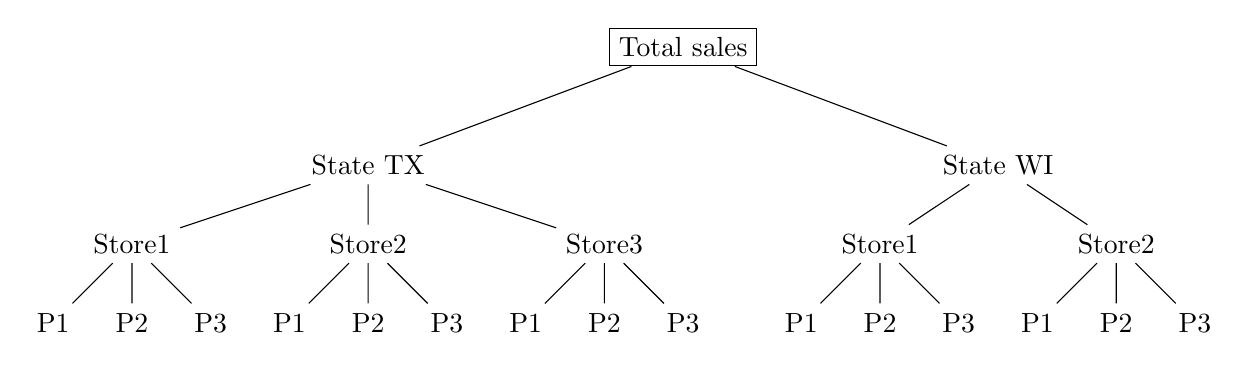
\begin{tikzpicture}
    [level 1/.style={sibling distance=80mm, level distance=15mm},
        level 2/.style={sibling distance=30mm, level distance=10mm},
        level 3/.style={sibling distance=10mm, level distance=10mm}]
        \node[rectangle,draw] {Total sales}
        child {node {State TX}
        child {node {Store1}
        child {node {P1}}
        child {node {P2}}
        child {node {P3}}
        }
        child {node {Store2}
        child {node {P1}}
        child {node {P2}}
        child {node {P3}}
        }
        child {node {Store3}
        child {node {P1}}
        child {node {P2}}
        child {node {P3}}
        }
        }
        child {node {State WI}
        child {node {Store1}
        child {node {P1}}
        child {node {P2}}
        child {node {P3}}
        }
        child {node {Store2}
        child {node {P1}}
        child {node {P2}}
        child {node {P3}}
        }
        };
    \end{tikzpicture}
    \caption{Hierarchical structure of product sales data (P1-3 = Product1-3)} \label{fig:hierarchical_structure}
\end{figure}




\subsection{Model implementation}\label{subsec:model-implementation}
The modelling approach is to build a single global on all series and exogenous variables for bottom-up aggregation.
For creating forecast models, the skforecast\cite{skforecast} library was used.
The base model for hierarchical forecasting was LightGBM~\cite{guolin_ke_highly_2017}
due to its efficiency and also because of its widespread usage in the M5 competition in this data set\cite{makridakis_m5_2022}.
Other ensemble models such as Random Forest or Gradient Boosting Machines could be used as well.
Other reasons for choosing LightGBM are that it can handle categorical variables without the need for one-hot encoding, and that it supports model-specific split and gain-based global feature importance methods.

Hyperparameter tuning was performed using the Optuna library\cite{optuna_2019}, by Bayesian optimisation.
The search space\ref{tab:hyperparam_search_space} was defined for the parameters of the LightGBM model, including the number of predictors, the minimum number of samples in the leaf, and the maximum depth of the tree.
In addition, the number of lagged sales records used as features was included in the search space.
For the search, the data was split into training and validation sets, the last year being the validation set used for backtesting.
The performance of the model was evaluated as a mean square error (MSE) in the validation set for each configuration.
The best configuration found was with 239 estimators and a maximum depth of 26 with a backtesting MSE 4263.01
The lagged sales records used as features were 1, 4, 5, 13, and 52 weeks.
\begin{table}
    \centering
    \begin{tabular}{|l|l|l|}
        \hline
        Parameter          & Search space & Description                                             \\
        \hline
        n\_estimators      & 50-1000      & Number of boosting iterations                           \\
        max\_depth         & 5-50         & Maximum depth of the tree                               \\
        min\_samples\_leaf & 1-10         & Minimum number of samples required to be at a leaf node \\
        num\_lagged\_sales & 4-52         & Number of lagged sales records used as features         \\
        \hline
    \end{tabular}
    \caption{Model hyperparameters search space}
    \label{tab:hyperparam_search_space}
\end{table}

The feature input for the final model is a table with the following columns:
\begin{itemize}
    \item week\_of\_year represented as numerical values (1-52)
    \item sell\_price for the week for the product in the store
    \item num\_of\_events for the week
    \item snap\_days for the week in the state
    \item lag\_\emph{n} for n in [1, 4, 5, 13, 52] representing the sales from the previous weeks
    \item series\_id noted as (\_level\_skforecast) encoded as a numerical value representing the series hierarchy
\end{itemize}
%\emph{Series\_id} could have been encoded as a one-hot encoded vector or as a categorical variable given it is supported by LightGBM.
%One-hot encoded vector would have increased the number of features and the complexity of the model,
%while with the categorical variable, the model would have been able to learn the hierarchy structure.



\section{Conclusions}
\label{sec:hierarchical_feature_importance_conclusions}
\input{chapters/05_feature_importance_hierarchy/04_conclusions}




\chapter{Collaborative development for decision support}
\label{ch:collaborative_development}

%\chapter{Collaborative Development for Decision Support}



\section{Best Practices for ML System Development}
\label{sec:best_practices_ml_system_development}
%https://www.researchgate.net/publication/372332486_Towards_Good_Practices_for_Collaborative_Development_of_ML-Based_Systems




\section{Automated delivery of models as services}
\label{sec:automated_delivery_models_services}
%https://www.cs.ubbcluj.ro/~studia-i/journal/journal/article/view/93/93



%

\section{Collaborative Development for Decision Support}
\label{sec:collaborative_development}
https://www.researchgate.net/publication/372332486_Towards_Good_Practices_for_Collaborative_Development_of_ML-Based_Systems





\section{Automated delivery of models as services}
%https://www.cs.ubbcluj.ro/~studia-i/journal/journal/article/view/93/93

Best Practices for Collaborative Development of ML Systems
\begin{itemize}
\item Insights from the development of a demand forecasting system.
\item Discussion on deploying scalable and interpretable ML models in industrial environments.
\end{itemize}





Best Practices for Collaborative Development of ML Systems
\begin{itemize}
    \item Insights from the development of a demand forecasting system.
    \item Discussion on deploying scalable and interpretable ML models in industrial environments.
\end{itemize}


%\section{Challenges in Deploying Explainable AI in Industry}
%\section{Conclusions}


\section{Conclusions}




\chapter{Conclusions and Future Work}
\label{ch:conclusions}

\section{Summary of Contributions}
\label{sec:summary_of_contributions}


\section{Future Research Directions}
\label{sec:future_research_directions}


    \appendix

    \setstretch{1}
    \bibliographystyle{apalike}
%    \bibliography{refs}
    \bibliography{biblography/explain}
    \label{bib}
    %\bibliography{file1,file2}


\end{document}

